%% =========================================================================
%% chapters/ch01-what-disease-is.tex
%%
%% Chapter 1. Derives, from one postulate, the objects the rest of the book
%% refers to: individuation against a medium, the cycle space of a reaction
%% network, holonomy, emergent cycles, maintenance, the viability set and
%% its margin, the three kinds of lesion, and the definition of disease.
%% Every link carries a label: [D] derived here, [S] supplied with a
%% reference, [C] checked on public data (validation/ch01/).
%%
%% Labels in this chapter are prefixed c1: to keep them apart from the
%% chapters that follow.
%% =========================================================================

\chapter{What Disease Is}
\label{ch:what-disease-is}

\begin{quote}
\itshape
La sant\'e c'est le luxe de pouvoir tomber malade et de s'en relever.
\upshape\medskip\\
\hfill --- Georges Canguilhem, \textit{Le normal et le pathologique} (1943)
\end{quote}

%% -------------------------------------------------------------------------
\section{The question}
\label{c1:sec-question}
%% -------------------------------------------------------------------------

Medicine has no definition of disease that a computation can use. It has a
list of diseases, a vocabulary for classifying them, and a working
agreement, renegotiated case by case, about which conditions belong on the
list. That is enough for clinical practice, which treats patients rather
than definitions. It is not enough for a book that intends to compute with
the word. Every later chapter will say that something is, or is not, a
disease, that one intervention removes it and another does not, that a
measurement can or cannot detect it. Each of those statements is only as
good as the definition it refers to, and this chapter supplies one.

The question is old and has three well-developed answers. The
\emph{biostatistical} answer of Boorse~\citep{boorse1977} says that a
disease is an internal state that reduces some function below the efficiency
typical of a reference class---people of the same age and sex. The
\emph{harmful dysfunction} answer of Wakefield~\citep{wakefield1992} adds
that the reduced function must be one the mechanism was selected for, and
that the reduction must be judged harmful by the standards of a society.
The third answer, which is older than both and which this chapter ends by
making precise, is Canguilhem's~\citep{canguilhem1989}: health is the
capacity of a living being to tolerate changes in its surroundings, to keep
living when its environment departs from the conditions it is used to, and
disease is the narrowing of that capacity. The epigraph is his: health is
the luxury of being able to fall ill and recover.

The first two answers need something outside the patient---a population
statistic, an evolutionary history, a social judgement. The third needs only
the patient and its surroundings. That is the property I want, for a reason
\Cref{c1:sec-postulate} makes exact: a bounded system cannot hold a complete
description of a system as complex as itself, so a definition of disease
that works by comparing a patient with a stored picture of health asks for
something no patient, cell or instrument can contain.

\subsection*{A correction to my own earlier answer}

In earlier versions of this work, including drafts of this book, I defined
disease as a loop with non-trivial holonomy: a cycle of reactions around
which the logarithms of the forward-to-backward rate ratios fail to sum to
zero. The word \emph{holonomy} was chosen deliberately and I keep it. But
the definition, in the form I gave it, cannot be right, and the reason is
instructive enough to organise the chapter around.

Stated precisely (\Cref{c1:sec-holonomy}), holonomy is the sum of an
edge quantity around a cycle. For the cycles that lie inside a reaction
network, that sum is zero by the first law of thermodynamics, in health and
in disease alike, and no enzyme defect can change it
(\Cref{c1:sec-internal}). For the cycles that pass through a network's
surroundings, the sum is \emph{not} zero, and it is not zero in any living
thing: it is the free energy the surroundings supply, and a system in which
every such sum vanished would be at equilibrium and could maintain nothing
(\Cref{c1:sec-medium,c1:sec-maintenance}). Non-trivial holonomy is
therefore the signature of being alive, not of being ill. What a disease
changes is not the holonomy but the currents it drives and the cycles that
exist to carry them (\Cref{c1:sec-viability,c1:sec-disease}). The human
erythrocyte, assembled from public databases, shows each step on real data
(\Cref{c1:sec-erythrocyte}).

\subsection*{How the chapter argues}

I follow the method of a derivation I have used elsewhere for a single
enzyme family: trace a chain of conditions from a minimal starting point to
the object of interest, and say at every link how strong the link is. Each
statement carries one or more labels:
\begin{itemize}[nosep]
\item \lnkD{} \emph{derived} here from the postulate and the definitions;
\item \lnkS{} \emph{supplied} from established physics, chemistry or
      medicine, with a reference;
\item \lnkC{} \emph{checked} here against public data, with the computation
      in \texttt{validation/ch01/}.
\end{itemize}
A derivation in this sense is a chain of necessary conditions and their
consequences. It does not claim that the conditions are sufficient for any
particular organism, and where the chain passes through a fact I can state
but not derive---that Gibbs energy is a state function, that an enzyme does
not move an equilibrium---I say so. \Cref{c1:sec-ledger} collects the labels.

%% -------------------------------------------------------------------------
\section{One postulate}
\label{c1:sec-postulate}
%% -------------------------------------------------------------------------

The starting point is a fact about records, not about matter.

\begin{definition}[Occupation, register, commitment]
\label{c1:def-commitment}
A system \emph{occupies} a state at each moment; occupation is not a record
and carries no cost in this accounting. A \emph{register} is a finite word
over an alphabet of $b\ge2$ letters. A \emph{commitment} is an event that
appends one letter to a register. The \emph{count} $M$ of a register is the
number of commitments made to it, overwrites included.
\end{definition}

\begin{postulate}[Counted commitment]
\label{c1:post-counted}
Every commitment costs at least a fixed amount $\theta>0$, and nothing but a
commitment changes a register.
\end{postulate}

\Cref{c1:post-counted} is the only physical assumption of the chapter;
everything else is definition, proof, or an input I label as supplied. Its
established counterpart is Landauer's bound: resetting one bit of a physical
memory in contact with a bath at temperature $T$ dissipates at least
$k_{\mathrm{B}}T\ln 2$~\citep{Landauer1961,bennett1982}, a bound since
approached in experiment~\citep{berut2012}. \lnkS{} I use $\theta$ abstractly
and never need its value.

The content of the postulate lies in the word \emph{fixed}. Positivity
alone would not do.

\begin{theorem}[Divergence along every selection]
\label{c1:thm-selection}
\lnkD{} Let $(c_i)_{i\ge1}$ be positive reals. Then $\inf_i c_i>0$ if and
only if $\sum_{i\in I}c_i=\infty$ for every infinite $I\subseteq\mathbb N$.
\end{theorem}

\begin{proof}
If $\vartheta=\inf_i c_i>0$, any $n$ terms sum to at least $n\vartheta$. If
$\inf_i c_i=0$, choose indices $i_1<i_2<\cdots$ with $c_{i_k}<2^{-k}$; that
selection sums to less than one.
\end{proof}

A process whose steps each cost at least $\theta$ therefore accumulates
cost without bound along any infinite subsequence of its steps; a process
whose steps are merely positive need not, since $\sum 2^{-i}=1$. With
\Cref{c1:post-counted}, the commitments made to a register are totally
ordered by their count and their cumulative cost satisfies $C_M\ge M\theta$
\lnkD. A system with a finite budget $B$ makes at most $\lfloor B/\theta
\rfloor$ commitments \lnkD.

The first use of the postulate is the reason disease cannot be defined
against a stored template.

\begin{proposition}[No complete self-template]
\label{c1:prop-template}
\lnkD{} Let a system have finitely many distinguishable states, and let a
register be one of its parts, so that its state set is $X=R\times Y$ with
$R$ the register's distinguishable states and $|Y|\ge2$. No map from $X$, or
from the state set of any system with as many states as $X$, into $R$ is
injective. In particular the register cannot hold a complete description of
the system it belongs to, or of any healthy counterpart of that system with
as many distinguishable states.
\end{proposition}

\begin{proof}
$|X|=|R|\,|Y|\ge2|R|>|R|$, and an injective map into $R$ would need
$|X|\le|R|$.
\end{proof}

That every state set here is finite is itself a consequence of the
postulate: a part with budget $B$ for binary distinctions distinguishes at
most $2^{\lfloor B/\theta\rfloor}$ configurations \lnkD. A cell, an
organism and an instrument can each hold partial descriptions of health---a
reference range, a consensus sequence---but not a complete one, and no
partial description fixes what counts as a deviation from it. Whatever
disease is, it must be computable from the system and its surroundings, and
any comparison it involves must be between two things an observer can hold
at once, not between a system and its own complete picture of itself.

%% -------------------------------------------------------------------------
\section{Individuation and the medium}
\label{c1:sec-individuation}
%% -------------------------------------------------------------------------

To say that a cell is diseased one must first be able to say what the cell
is: where it ends and its surroundings begin. The measure of that boundary
used throughout this book is the cheapest way of cutting a thing off.

\begin{definition}[Contact graph, separation cost]
\label{c1:def-contact}
A \emph{contact graph} is a finite connected graph $G=(V,E,w)$ with weights
$w:E\to(0,\infty)$ and a distinguished vertex $m$, the \emph{medium}. For
$S\subseteq V$ write $\partial S$ for the set of edges with exactly one end
in $S$. The \emph{separation cost} of $v\ne m$ is
\begin{equation}
\sigma_G(v)=\min\{\,w(\partial S): v\in S\subseteq V\setminus\{m\}\,\}.
\label{c1:eq-sep}
\end{equation}
A minimiser is an \emph{identity region} of $v$. Weights are \emph{counted}
if they are positive integers.
\end{definition}

The weight of an edge is the cost of separating its ends, never a distance
between them; separation costs add along a cut, distances do not. By the
max-flow min-cut theorem~\citep{fordfulkerson1956} $\sigma_G(v)$ is the
value of a maximum flow from $v$ to $m$, so it is computable in polynomial
time. \lnkS

\begin{theorem}[Floor and monotonicity]
\label{c1:thm-floor}
\lnkD{} (a) With counted weights, $\sigma_G(v)\ge\lambda_G(v,m)\ge1$, where
$\lambda_G(v,m)$ is the largest number of edge-disjoint paths from $v$ to
$m$. (b) If $G'\supseteq G$ is obtained by adding vertices and edges and
leaving existing weights unchanged, then $\sigma_{G'}(v)\ge\sigma_G(v)$.
(c) With positive real weights, no lower bound independent of the graph
survives such additions.
\end{theorem}

\begin{proof}
(a) Each of $\lambda_G(v,m)$ edge-disjoint paths crosses every cut
separating $v$ from $m$~\citep{menger1927}, and each crossing edge weighs at
least one; connectivity gives $\lambda_G\ge1$. (b) Let $S'$ attain
$\sigma_{G'}(v)$ and put $S=S'\cap V$. Every edge of $G$ leaving $S$ also
leaves $S'$, so $\sigma_G(v)\le w(\partial_G S)\le w(\partial_{G'}S')$.
(c) Add at step $k$ a vertex joined to $v$ and to $m$ by edges of weight
$1/k$: its separation cost is at most $2/k$.
\end{proof}

\begin{proposition}[Identity is a region]
\label{c1:prop-region}
\lnkD{} There are contact graphs in which every identity region of some $v$
contains a vertex other than $v$.
\end{proposition}

\begin{proof}
Take $v,u,m$ with $w(v,u)=10$, $w(v,m)=3$, $w(u,m)=1$. Then
$w(\partial\{v\})=13$ and $w(\partial\{v,u\})=4$, and these are the only
candidate sets.
\end{proof}

Two things in this section are needed later. The first is that what a
thing is, measured by how it is cut from its surroundings, is settled
together with some of its neighbours: a cell is not the sum of separately
individuated molecules. The second is the medium itself. In a contact graph
it is a single vertex, a structural slot for whatever an item is
distinguished against. \Cref{c1:sec-medium} gives that slot content: for a
cell, the medium is the plasma or culture fluid that holds glucose, oxygen,
lactate and ions at concentrations the cell does not set. The same vertex
$m$ will close the cell's reactions into cycles, and the holonomy of those
cycles will turn out to be the medium's contribution to the cell's life.

%% -------------------------------------------------------------------------
\section{Cycles and holonomy}
\label{c1:sec-holonomy}
%% -------------------------------------------------------------------------

This section defines, with nothing assumed beyond linear algebra, the
objects the phrase \emph{loop holonomy} refers to. Readers who know the
cycle space of a graph will find nothing new in it except the passage from
graphs to reaction networks, which is where my earlier usage went wrong.

\subsection{Graphs}

Let $\Gamma=(V,E)$ be a finite directed graph with $n$ vertices and $r$
edges. Its \emph{incidence matrix} $B\in\mathbb Z^{n\times r}$ has $B_{ve}=-1$
if edge $e$ leaves $v$, $+1$ if it enters $v$, and $0$ otherwise.

\begin{definition}[Cycle space]
\label{c1:def-cycles}
The \emph{cycle space} of $\Gamma$ is $Z(\Gamma)=\ker B\subseteq\mathbb R^r$.
A \emph{cycle} is an element of $Z(\Gamma)$; an \emph{integer cycle} is one in
$\mathbb Z^r$. Its dimension $\beta_1=r-\operatorname{rank}B$ is the first
Betti number of $\Gamma$.
\end{definition}

A closed walk that traverses edge $e$ forwards $a_e$ times and backwards
$b_e$ times defines the integer vector $z_e=a_e-b_e$, which lies in $\ker B$
because every vertex is entered as often as it is left. Conversely the
integer cycles are spanned by such walks~\citep{biggs1993}. For a connected
graph $\operatorname{rank}B=n-1$, so $\beta_1=r-n+1$. \lnkS{} The cycle
space is a \emph{topological} object in the precise sense that it depends
only on which vertices the edges join, not on any number attached to them.

\begin{definition}[Cochains, coboundary]
\label{c1:def-cochain}
A \emph{0-cochain} is a function $\phi:V\to\mathbb R$, a vector in
$\mathbb R^n$; a \emph{1-cochain} is a function $\omega:E\to\mathbb R$, a
vector in $\mathbb R^r$. The \emph{coboundary} of a 0-cochain is the
1-cochain $\delta\phi=B^{\mathsf T}\phi$, whose value on an edge from $u$ to
$v$ is $\phi(v)-\phi(u)$. A 1-cochain is \emph{exact} if it is a coboundary.
\end{definition}

\begin{definition}[Holonomy]
\label{c1:def-holonomy}
The \emph{holonomy} of a 1-cochain $\omega$ around a cycle $z$ is
\begin{equation}
\operatorname{hol}_\omega(z)=\langle\omega,z\rangle=\sum_{e\in E}z_e\,\omega_e .
\label{c1:eq-hol}
\end{equation}
The holonomy is \emph{trivial} if $\operatorname{hol}_\omega(z)=0$ for every
$z\in Z(\Gamma)$.
\end{definition}

For a closed walk, \Cref{c1:eq-hol} is the sum of $\omega$ along the walk,
counting backward traversals negatively: the total change accumulated by
going round and coming back. That is what the word means in geometry,
where a connection transports a vector along a path and the holonomy of a
loop is the transformation the vector has undergone on its return.

\begin{theorem}[Trivial holonomy is exactness]
\label{c1:thm-exact}
\lnkD{} A 1-cochain has trivial holonomy if and only if it is exact. It
suffices to check the holonomy on a basis of $Z(\Gamma)$, and a basis of
integer cycles exists.
\end{theorem}

\begin{proof}
In finite dimensions $\operatorname{im}B^{\mathsf T}=(\ker B)^{\perp}$, so
$\omega\perp Z(\Gamma)$ if and only if $\omega=B^{\mathsf T}\phi$ for some
$\phi$. Holonomy is linear in $z$, so vanishing on a basis gives vanishing
everywhere. Since $B$ has integer entries, Gaussian elimination over the
rationals gives a rational basis of $\ker B$, which can be scaled to integers.
\end{proof}

\begin{remark}[Group-valued holonomy]
\label{c1:rem-group}
A \emph{connection} with values in a group $\mathcal G$ assigns an element
$g_e\in\mathcal G$ to each edge, and the holonomy of a closed walk is the
ordered product of the $g_e$ along it. For $\mathcal G=(\mathbb R,+)$ this is
\Cref{c1:eq-hol}. For the positive reals under multiplication---a ratio of
rate constants on each edge---it is the product of the ratios, and taking
logarithms returns \Cref{c1:eq-hol}. Non-commuting groups give holonomies
that \Cref{c1:eq-hol} does not capture, and in earlier work I wrote the
holonomy of a loop as a composition of \emph{constraint maps} to leave room
for them. Nothing in thermodynamic data requires that room, and the next
subsection shows that for reaction networks only the additive form is even
defined.
\end{remark}

\subsection{Reaction networks}

A reaction is not an edge. It may consume two species and produce three, so
a reaction network is a hypergraph, and a closed walk through it is not
defined. What survives is the linear algebra.

\begin{definition}[Reaction network]
\label{c1:def-network}
A \emph{reaction network} has a finite set $\mathcal S$ of $n$ species, a
finite set $\mathcal R$ of $r$ reactions, and a \emph{stoichiometric matrix}
$N\in\mathbb Z^{n\times r}$ whose entry $N_{ie}$ is the net number of
molecules of species $i$ produced when reaction $e$ runs once forwards.
Its \emph{cycle space} is $Z(N)=\ker N$, of dimension $r-\operatorname{rank}N$.
\end{definition}

A graph is the special case $N=B$, in which every reaction converts one
molecule of one species into one molecule of another. Every definition and
every proof above was written in terms of the matrix alone, so all of them
carry over with $B$ replaced by $N$: cochains on species and on reactions,
the coboundary $\delta\phi=N^{\mathsf T}\phi$, holonomy as
$\langle\omega,z\rangle$ for $z\in\ker N$, and \Cref{c1:thm-exact} with the
same proof. \lnkD{} A cycle of a reaction network is a combination of
reactions, run forwards or backwards an integer number of times each, after
which every species is restored. Each run of a reaction is a discrete event,
so an integer cycle is a counted object in the sense of
\Cref{c1:post-counted}: a turn of a cycle can be committed, and its holonomy
is the change accumulated per turn.

The one fact about cycles that the rest of the chapter uses most is what
they say about steady flux.

\begin{proposition}[Only reactions on a cycle carry steady flux]
\label{c1:prop-flux}
\lnkD{} Let $N_{\mathcal I}$ be the rows of $N$ for a set $\mathcal I$ of
species whose amounts must not change, and let $F=\ker N_{\mathcal I}$. A
net flux vector $J\in\mathbb R^r$ keeps every species of $\mathcal I$ at
steady state if and only if $J\in F$. Reaction $e$ carries a non-zero flux
in some such $J$ if and only if deleting column $e$ from $N_{\mathcal I}$
leaves its rank unchanged.
\end{proposition}

\begin{proof}
The rate of change of the amounts of the species of $\mathcal I$ is
$N_{\mathcal I}J$, which vanishes exactly when $J\in F$. Write
$N_{\mathcal I}^{-e}$ for $N_{\mathcal I}$ without column $e$; its kernel is
isomorphic to $F_e=\{z\in F:z_e=0\}$. If the rank is unchanged,
$\dim F_e=(r-1)-\operatorname{rank}N_{\mathcal I}=\dim F-1$, so the linear
functional $z\mapsto z_e$ is not zero on $F$. If the rank falls by one,
$\dim F_e=\dim F$, so $F_e=F$ and $z_e=0$ for every $z\in F$.
\end{proof}

When $\mathcal I$ is every species, $F=Z(N)$. In general $F$ is larger, and
\Cref{c1:sec-medium} is about the difference. A reaction that lies on no
cycle of $F$ carries no flux at any steady state, however active its enzyme:
it can matter only transiently, while something is being built up or run
down.

%% -------------------------------------------------------------------------
\section{Holonomy inside a network vanishes}
\label{c1:sec-internal}
%% -------------------------------------------------------------------------

Now attach numbers to the reactions. Three thermodynamic 1-cochains are in
use: the reaction Gibbs energy $\Delta_rG$, its standard value
$\Delta_rG^{\circ}$ (or the transformed $\Delta_rG'^{\circ}$ of biochemistry,
at fixed pH, ionic strength and pMg~\citep{alberty2003}), and the logarithm
of an equilibrium constant or of a forward-to-backward rate-constant ratio.
The definition of disease I am correcting used the last.

\begin{inputstmt}[State function]
\label{c1:in-state}
\lnkS{} In a system held at one temperature and pressure, each species $i$
has a chemical potential $\mu_i$, and the Gibbs energy of reaction $e$ is
$\Delta_rG_e=\sum_i N_{ie}\mu_i$; for a dilute species
$\mu_i=\mu_i^{\circ}+RT\ln a_i$~\citep{kondepudi1998,alberty2003}. The same
holds for transformed potentials $\mu_i'$ at fixed pH, with protons removed
from the stoichiometry~\citep{alberty2003}.
\end{inputstmt}

In the language of \Cref{c1:sec-holonomy}, \Cref{c1:in-state} says that
$\Delta_rG=N^{\mathsf T}\mu=\delta\mu$: the reaction Gibbs energy is the
coboundary of the chemical potential. The consequence is immediate, and it
is the hinge of the chapter.

\begin{theorem}[Internal holonomy vanishes]
\label{c1:thm-internal}
\lnkD{} For every cycle $z\in\ker N$, at any concentrations and any enzyme
levels,
\begin{equation}
\operatorname{hol}_{\Delta_rG}(z)=\langle N^{\mathsf T}\mu,z\rangle
=\langle\mu,Nz\rangle=0 .
\label{c1:eq-internal}
\end{equation}
The same holds for $\Delta_rG^{\circ}$, for $\Delta_rG'^{\circ}$, and for
$\ln K_e=-\Delta_rG^{\circ}_e/RT$.
\end{theorem}

\begin{proof}
$Nz=0$. The standard and transformed values are coboundaries of $\mu^{\circ}$
and $\mu'^{\circ}$ by \Cref{c1:in-state}.
\end{proof}

The statement about equilibrium constants is Wegscheider's
condition~\citep{Wegscheider1901}. It carries over to rate constants
through two further inputs.

\begin{inputstmt}[Detailed balance, catalysis]
\label{c1:in-haldane}
\lnkS{} For an elementary reaction with mass-action rate constants $k^+_e$
and $k^-_e$, $k^+_e/k^-_e=K_e$; for an enzyme-catalysed reaction the
corresponding kinetic parameters satisfy the Haldane relation, so a catalyst
changes forward and backward rates in the same proportion and leaves $K_e$
unchanged~\citep{haldane1930,Wegscheider1901}.
\end{inputstmt}

\begin{corollary}[The rate-constant holonomy vanishes]
\label{c1:cor-rates}
\lnkD{} For every $z\in\ker N$,
$\sum_e z_e\ln(k^+_e/k^-_e)=\sum_e z_e\ln K_e=0$. No change in the amount,
activity or kinetic constants of any enzyme changes this sum.
\end{corollary}

This is the quantity I called the log-holonomy of a loop and defined disease
to make non-zero. \Cref{c1:cor-rates} says that on any cycle internal to a
network it is zero whatever the network's state, healthy or not, and that no
enzyme lesion can make it otherwise. A loss-of-function allele slows both
directions of the reaction it affects by the same factor, and so does a
gain of function; neither moves the ratio. My earlier definition, applied
to internal cycles, classified every cell as healthy.

\subsection*{What a non-zero internal sum means}

Then what does a computed non-zero sum mean? It means the numbers were not
all measured on one system---they came from different laboratories,
conditions or methods, and they disagree. \Cref{c1:thm-internal} turns this
into a test of data, and the test can be run.

\paragraph{Check on measured equilibrium constants.} \lnkC{} The NIST
Thermodynamics of Enzyme-Catalyzed Reactions Database
(TECRDB)~\citep{goldberg2004} records apparent equilibrium constants measured
one reaction at a time, so its values are not differences of formation
energies and nothing forces their cycle sums to zero. In the snapshot used
in this book, $3{,}276$ measurements at $293$--$313$~K of evaluation grade
A--C, from $908$ studies of $418$ reactions, were transformed to a common
reference state as component contribution prepares its training
data~\citep{beber2022}. Their stoichiometry has a cycle space of dimension
$67$, and every basis cycle sums to between $0.04$ and $27.8$~kJ/mol. Each
sum was compared with the uncertainty propagated from the measurements on
its edges (one study, one value; scatter pooled over reactions measured in
several studies, $2.7$~kJ/mol). Sixty of the $67$ sums cannot be
distinguished from zero; seven exceed the $99$th percentile of a Gaussian
error model, three exceed the $99$th percentile of the error actually
observed between repeated measurements of one reaction, and none exceeds a
distribution-free (Chebyshev) bound. Restricted to grade-A measurements,
$13$ cycles remain and two exceed the bound. The cycles that exceed it share
individual measurements---one constant for pyrophosphate-dependent
phosphofructokinase lies on a flagged cycle in $94\%$ of $200$ randomly
chosen cycle bases---which is what a defect in a datum, and not in a cell,
looks like. The full analysis is experiment R1 of the companion paper on
cycle-test tolerances, from which these numbers are taken.

So the data agree with \Cref{c1:thm-internal} as far as they can: the
internal cycle sums of real measurements are measurement error, of a size
and with tails one can calibrate. I draw the conclusion plainly. \emph{A
non-zero internal holonomy is a property of a dataset, never of a cell.} A
cycle-consistency test on internal cycles is a quality check on
thermodynamic data, and a useful one, but it cannot detect disease, because
the quantity it tests is fixed by physics.

%% -------------------------------------------------------------------------
\section{The medium closes the network}
\label{c1:sec-medium}
%% -------------------------------------------------------------------------

A cell is not a closed flask. Glucose arrives from the plasma faster than
the cell can deplete it, lactate leaves faster than it can accumulate, and
the plasma, not the cell, sets their concentrations. The medium of
\Cref{c1:sec-individuation} is exactly this: what an item is distinguished
against, and what it exchanges with.

\begin{inputstmt}[Reservoir]
\label{c1:in-reservoir}
\lnkS{} The species of a network divide into \emph{internal} species
$\mathcal I$, whose amounts the system's own reactions determine, and
\emph{exchanged} species $\mathcal X$, whose chemical potentials
$\mu_{\mathcal X}$ the medium holds fixed independently of the system. In
nonequilibrium thermodynamics the exchanged species are said to be
\emph{chemostatted}~\citep{polettini2014}.
\end{inputstmt}

Split the stoichiometric matrix into the rows for internal species and the
rows for exchanged species, $N_{\mathcal I}$ and $N_{\mathcal X}$. By
\Cref{c1:prop-flux} the steady fluxes of the open system form the space
$F=\ker N_{\mathcal I}$, which contains the cycle space $Z=\ker N$ of the
closed one.

\begin{definition}[Emergent cycles]
\label{c1:def-emergent}
An element of $F$ is a \emph{cycle through the medium}. Its \emph{exchange}
is $N_{\mathcal X}z$, the net amount of each exchanged species the system
produces per turn. A cycle through the medium with non-zero exchange is
\emph{emergent}; the internal cycles are those of $Z$, whose exchange is
zero.
\end{definition}

\begin{proposition}[Counting emergent cycles]
\label{c1:prop-count}
\lnkD{} $\dim F-\dim Z=\operatorname{rank}N-\operatorname{rank}N_{\mathcal I}$.
\end{proposition}

\begin{proof}
$\dim F=r-\operatorname{rank}N_{\mathcal I}$ and
$\dim Z=r-\operatorname{rank}N$.
\end{proof}

In a graph the construction is literal. Join every exchanged vertex to the
medium vertex $m$: a pathway that takes something from the medium and
returns something else to it becomes a closed loop through $m$. The vertex
that individuated the cell in \Cref{c1:sec-individuation} is the vertex that
closes its metabolism.

\begin{example}[Five reactions]
\label{c1:ex-toy}
Species $X,A,B,C,Y$; reactions $e_1\colon X\to A$, $e_2\colon A\to B$,
$e_3\colon B\to C$, $e_4\colon C\to A$, $e_5\colon C\to Y$. With every
species internal the network is a connected graph on five vertices with five
edges, so $\dim Z=1$, spanned by $z_0=e_2+e_3+e_4$, and $e_1,e_5$ lie on no
cycle: at steady state they carry nothing. Declare $X$ and $Y$ exchanged.
Then $\operatorname{rank}N_{\mathcal I}=3$, $\dim F=2$, and $F$ gains the
emergent cycle $z_1=e_1+e_2+e_3+e_5$, with exchange $X\to Y$. By
\Cref{c1:in-state},
\[
\operatorname{hol}(z_0)=0,\qquad
\operatorname{hol}(z_1)=\mu_Y-\mu_X .
\]
\end{example}

The example generalises to the theorem that replaces my earlier definition.

\begin{theorem}[The medium sets the holonomy]
\label{c1:thm-medium}
\lnkD{} For every cycle through the medium $z\in F$,
\begin{equation}
\operatorname{hol}_{\Delta_rG}(z)
=\langle\mu_{\mathcal X},N_{\mathcal X}z\rangle ,
\label{c1:eq-medium}
\end{equation}
the Gibbs energy of the cycle's net exchange at the medium's chemical
potentials. It does not depend on the concentrations of internal species,
on the amount or kinetics of any enzyme, or on which path through the
network the cycle takes.
\end{theorem}

\begin{proof}
$\langle N^{\mathsf T}\mu,z\rangle=\langle\mu,Nz\rangle
=\langle\mu_{\mathcal I},N_{\mathcal I}z\rangle+
\langle\mu_{\mathcal X},N_{\mathcal X}z\rangle$, and $N_{\mathcal I}z=0$.
\end{proof}

\Cref{c1:thm-internal} is the case $N_{\mathcal X}z=0$. So the holonomy of
every cycle is fixed by something the system does not control: by physics
for internal cycles, by the medium for emergent ones. The system controls
two other things: which cycles exist, through the reactions it catalyses,
and how much current each carries, through how fast it catalyses them. The
rest of the chapter is about those two.

\paragraph{Check on the erythrocyte.} \lnkC{} The mature human red cell has
no nucleus and no mitochondria and lives on glycolysis~\citep{grace2018}, so
its metabolism is small enough to assemble from annotation alone. Its
network was built from the catalytic activities that UniProtKB/Swiss-Prot
records for $38$ erythrocyte enzymes and pumps~\citep{uniprot2025}, each
expanded into its Rhea reactions~\citep{bansal2022}
(\Cref{c1:sec-erythrocyte} gives the details). With every species internal,
as in a closed flask, it has $75$ distinct reactions and a cycle space of
dimension $7$, and only $19$ reactions lie on any cycle. Pyruvate kinase is
not one of them, nor are hexokinase, phosphofructokinase or lactate
dehydrogenase: by \Cref{c1:prop-flux} the closed network could not run
glycolysis at all. Let the medium hold three species, glucose, lactate and
water. One emergent cycle appears, and every glycolytic enzyme lies on it
(\Cref{c1:fig-ery}, second column). Its exchange is glucose $\to$ 2
lactate, and its holonomy, computed with component
contribution~\citep{beber2022} at erythrocyte conditions (pH $7.2$, ionic
strength $0.15$~M, $37\,^{\circ}$C), is
$\Delta_rG'^{\circ}=-198.6\pm1.9$~kJ/mol, or $-220.6$~kJ/mol at plasma
glucose $5$~mM and lactate $1$~mM. The cell captures two ATP per turn, each
worth $\Delta_rG'^{\circ}=-29.4$~kJ/mol of hydrolysis. No enzyme in the cell
can change the $-220.6$; only the plasma can.

%% -------------------------------------------------------------------------
\section{No holonomy, no maintenance}
\label{c1:sec-maintenance}
%% -------------------------------------------------------------------------

A cycle with zero holonomy can be traversed, but nothing pushes anything
round it. To make that precise one needs the relation between a reaction's
Gibbs energy and the direction of its flux.

\begin{inputstmt}[Flux--force relation]
\label{c1:in-fluxforce}
\lnkS{} Each reaction $e$ runs forwards and backwards at one-way rates
$J^+_e,J^-_e>0$, with
$\ln(J^+_e/J^-_e)=-\Delta_rG_e/RT$~\citep{beardqian2007}. Hence the net flux
$J_e=J^+_e-J^-_e$ has the sign of $-\Delta_rG_e$, and $J_e=0$ exactly when
$\Delta_rG_e=0$.
\end{inputstmt}

Write $\Pi=-\sum_e J_e\,\Delta_rG_e$ for the rate at which a steady state
dissipates Gibbs energy. By \Cref{c1:in-fluxforce} each term is
non-negative and vanishes only if $J_e=0$. \lnkD

\begin{theorem}[No holonomy, no current]
\label{c1:thm-nocurrent}
\lnkD{} At a steady state $J\in F$,
\begin{equation}
\Pi=-\operatorname{hol}_{\Delta_rG}(J)
=-\langle\mu_{\mathcal X},N_{\mathcal X}J\rangle .
\label{c1:eq-power}
\end{equation}
If the holonomy of every cycle through the medium vanishes, then $J=0$.
\end{theorem}

\begin{proof}
$\Pi=-\langle\Delta_rG,J\rangle=-\operatorname{hol}_{\Delta_rG}(J)$ because
$J\in F$, and \Cref{c1:thm-medium} gives the second form. If every holonomy
on $F$ vanishes then $\Pi=0$; a sum of non-negative terms that is zero has
every term zero, so every $J_e=0$.
\end{proof}

The second form of \Cref{c1:eq-power} says that everything the steady state
dissipates is drawn from the medium: $-N_{\mathcal X}J$ is the rate at which
the system takes up each exchanged species, and $\Pi$ is the Gibbs energy
those uptakes carry in. Expanding $J$ on a basis of $F$ gives Schnakenberg's
decomposition of entropy production into cycle currents times cycle
affinities~\citep{schnakenberg1976}, and \Cref{c1:thm-internal} says the
internal cycles contribute nothing to it. \lnkS{} One more consequence is
worth stating, because it is easy to get wrong.

\begin{corollary}[Loop law]
\label{c1:cor-loop}
\lnkD{} No steady state carries a current around an internal cycle: there
is no non-zero $z\in Z$ whose support lies in the support of $J$ and whose
signs agree with those of $J$ there.
\end{corollary}

\begin{proof}
For such a $z$, each term $z_e\Delta_rG_e$ with $z_e\ne0$ has the sign of
$J_e\Delta_rG_e<0$, so $\operatorname{hol}(z)<0$, contradicting
\Cref{c1:thm-internal}.
\end{proof}

This is the thermodynamic loop law of Qian and Beard~\citep{qianbeard2005}.
Internal cycles in a living network are parallel routes between the same
endpoints, both run forwards; they are never wheels that turn.

Now connect this to \Cref{c1:post-counted}. A living cell is not merely
individuated, as a crystal is; its individuation decays. Ion gradients leak,
glutathione is oxidised, proteins are damaged, and left alone the cell
relaxes to equilibrium with its medium~\citep{schrodinger1944,kondepudi1998},
at which point the gradients and redox ratios that distinguish it from the
plasma are gone. \lnkS{} What keeps it distinct is repair, and repair is a
sequence of discrete events---a sodium ion pumped out, a disulfide reduced,
a protein replaced---each of which writes the cell's state back.

\begin{definition}[Maintained individuation]
\label{c1:def-maintained}
A system is \emph{maintained} if its identity region with respect to the
medium (\Cref{c1:def-contact}) would not persist at equilibrium with that
medium, and persists by commitments made at a positive steady rate $\nu$.
\end{definition}

\begin{inputstmt}[The cost of a commitment is dissipated]
\label{c1:in-landauer}
\lnkS{} The cost $\theta$ of each commitment of \Cref{c1:post-counted} is
paid as dissipated Gibbs energy, in the sense of
Landauer~\citep{Landauer1961,bennett1982}, and is part of $\Pi$.
\end{inputstmt}

\begin{theorem}[Maintenance needs emergent holonomy]
\label{c1:thm-maintenance}
\lnkD{} A maintained system dissipates $\Pi\ge\nu\theta>0$ at steady state.
Consequently it has at least one emergent cycle with non-zero holonomy, it
carries a non-zero current, and the power it spends is drawn entirely from
its medium.
\end{theorem}

\begin{proof}
$\Pi\ge\nu\theta$ by \Cref{c1:in-landauer}, and $\nu\theta>0$. By
\Cref{c1:thm-nocurrent}, if every holonomy on $F$ vanished then $J=0$ and
$\Pi=0$. So some $z\in F$ has non-zero holonomy, by \Cref{c1:thm-internal}
it is not in $Z$, and $J\neq0$. The power is \Cref{c1:eq-power}.
\end{proof}

This is the inversion promised at the start. A system in which every
holonomy is trivial, internal and emergent, is at equilibrium with its
medium, carries no current, and maintains nothing: it is dead, or was never
alive. Non-trivial holonomy on emergent cycles is a precondition of life.
Holonomy is the right object, but it measures what the medium supplies, not
what has gone wrong.

%% -------------------------------------------------------------------------
\section{Viability, margin and lesion}
\label{c1:sec-viability}
%% -------------------------------------------------------------------------

A system that needs current to persist can fail to get enough. Whether it
does depends on two things: the medium, which sets the holonomies, and the
system, which sets which cycles exist and how readily they conduct. The
viability of a system is the set of media in which the second suffices for
the first.

\begin{definition}[System]
\label{c1:def-kinetic}
A \emph{system} $\mathcal N=(N,\kappa)$ is a reaction network $N$ together
with kinetic parameters $\kappa$: for each reaction, the constants that fix
its one-way rates as functions of concentrations. The exchanged species
$\mathcal X$ and a set $\mathcal M\subseteq\mathbb R^{\mathcal X}$ of
admissible medium states $\mu_{\mathcal X}$ are fixed.
\end{definition}

\begin{inputstmt}[Steady state, demand]
\label{c1:in-steady}
\lnkS{} For each $\mu_{\mathcal X}\in\mathcal M$ the system relaxes to a
steady state with net flux $J_{\mathcal N}(\mu_{\mathcal X})\in F$. Its
maintenance requires a set $\mathcal D\subseteq\mathbb R^{r}$ of adequate
fluxes---for instance, sodium pumped out at least as fast as it leaks
in~\citep{grace2018}. Both are properties of a particular organism; this
chapter assumes them and does not compute them.
\end{inputstmt}

\begin{definition}[Viability set, margin]
\label{c1:def-viability}
The \emph{viability set} of $\mathcal N$ is
\[
\mathcal V(\mathcal N)=\{\mu_{\mathcal X}\in\mathcal M :
J_{\mathcal N}(\mu_{\mathcal X})\in\mathcal D\}.
\]
$\mathcal N$ is \emph{alive} in $\mu_{\mathcal X}$ if
$\mu_{\mathcal X}\in\mathcal V(\mathcal N)$. Writing $B_\rho(\mu_{\mathcal
X})$ for the media with $\max_x|\mu'_x-\mu_x|\le\rho$, the \emph{margin} of
$\mathcal N$ in $\mu_{\mathcal X}$ is
\[
h(\mathcal N,\mu_{\mathcal X})=\sup\{\rho\ge0:
B_\rho(\mu_{\mathcal X})\cap\mathcal M\subseteq\mathcal V(\mathcal N)\},
\]
taken as zero when the set is empty.
\end{definition}

The margin is measured in the units of chemical potential, kJ/mol. It is
computed from the system and its medium alone, with no reference to a
population, a template or a history: it says how far the medium can move,
in its worst direction, before the system can no longer keep itself going.
It is Canguilhem's tolerance of the inconstancies of the
environment~\citep{canguilhem1989}, given a number.

Systems change, and a reaction network can change in only a few ways.

\begin{definition}[Lesion]
\label{c1:def-lesion}
A \emph{lesion} is a change $\lambda\colon\mathcal N\to\mathcal N'$ of one of
three kinds, or a composition of them:
\begin{enumerate}[label=(L\arabic*),nosep]
\item \emph{deletion} of a reaction (deleting a species deletes every
      reaction it takes part in);
\item \emph{addition} of a reaction, with any new species it brings;
\item \emph{conductance change}: a change of $\kappa$ with $N$ fixed.
\end{enumerate}
\end{definition}

That every change of a system is such a composition is immediate: compare
the two reaction sets, delete what is missing, add what is new, and adjust
the kinetics of the rest. \lnkD{} An allele that abolishes an enzyme is
(L1); one that lowers its activity is (L3); a toxin, a leaking channel or a
pathogen's enzymes are (L2). What a lesion can and cannot do follows from
the earlier sections.

\begin{theorem}[What a lesion changes]
\label{c1:thm-lesion}
\lnkD{} Let $\lambda\colon\mathcal N\to\mathcal N'$ keep the exchanged
species $\mathcal X$.
\begin{enumerate}[label=(\alph*),nosep]
\item No lesion changes the holonomy of any cycle that $\mathcal N$ and
      $\mathcal N'$ share: internal cycles have holonomy zero in both, and
      emergent ones have holonomy
      $\langle\mu_{\mathcal X},N_{\mathcal X}z\rangle$ in both.
\item A conductance change (L3) leaves $Z$, $F$ and every holonomy
      unchanged; it changes only the currents.
\item Deleting reaction $e$ (L1) lowers $\dim F$ by one if $e$ lies on a
      cycle of $F$. If it does not, $F$ is unchanged, every steady state of
      $\mathcal N$ is a steady state of $\mathcal N'$, and, when steady
      states are unique, $\mathcal V(\mathcal N')=\mathcal V(\mathcal N)$.
\item Adding a reaction (L2) raises $\dim F$ by at most one, and the
      holonomy of any new emergent cycle is fixed by the medium.
\end{enumerate}
\end{theorem}

\begin{proof}
(a) is \Cref{c1:thm-internal,c1:thm-medium}, which involve only $N$ and
$\mu_{\mathcal X}$. (b) $Z$ and $F$ depend on $N$ alone. (c) The dimension
count is \Cref{c1:prop-flux}. If $e$ lies on no cycle of $F$, every steady
flux of $\mathcal N$ has $J_e=0$, so at the same concentrations the
remaining reactions still balance every internal species and the state is
steady for $\mathcal N'$; uniqueness then gives
$J_{\mathcal N'}=J_{\mathcal N}$ in every medium, hence the same viability
set when $\mathcal D$ does not involve $e$. (d) Adding a column raises the
dimension of a kernel by at most one; the holonomy is \Cref{c1:thm-medium}.
\end{proof}

\begin{corollary}[Where a lesion acts depends on the medium]
\label{c1:cor-medium}
\lnkD{} Whether a reaction lies on a cycle of $F=\ker N_{\mathcal I}$
depends on which species the medium exchanges. A deletion that leaves
viability unchanged under one exchanged set can change it under another.
\end{corollary}

\begin{proof}
$N_{\mathcal I}$ is $N$ with the rows of $\mathcal X$ removed, so its rank,
and the rank test of \Cref{c1:prop-flux}, depend on $\mathcal X$.
\Cref{c1:ex-toy} has $e_1$ and $e_5$ off every cycle with no medium and on
one with $\{X,Y\}$ exchanged. Part (c) of \Cref{c1:thm-lesion} applies to
their deletion under the first exchanged set and not under the second.
\end{proof}

%% -------------------------------------------------------------------------
\section{Disease}
\label{c1:sec-disease}
%% -------------------------------------------------------------------------

Everything is now in place to state the definition the rest of the book
refers to.

\begin{definition}[Disease]
\label{c1:def-disease}
Fix the exchanged species and a set $\mathcal M$ of media. A lesion
$\lambda\colon\mathcal N\to\mathcal N'$ is \emph{pathogenic} on
$\mathcal M$ if it narrows the viability set,
\[
\mathcal V(\mathcal N')\subsetneq\mathcal V(\mathcal N),
\]
and its \emph{severity} in a medium $\mu_{\mathcal X}$ is the loss of margin
$h(\mathcal N,\mu_{\mathcal X})-h(\mathcal N',\mu_{\mathcal X})$. A system
$\mathcal N'$ is \emph{diseased with respect to} $\mathcal N$ if it differs
from $\mathcal N$ by a pathogenic lesion. A system is \emph{dead} in a
medium outside its viability set.
\end{definition}

Six remarks fix what the definition says.

\emph{Disease is a relation.} The definition compares two systems, the
lesioned one and the one it differs from. It is not a property of a single
state, and \Cref{c1:prop-template} says why it cannot be: a single system
cannot contain the other term of the comparison. The second term is a
network an observer can write down---the same pathway with the reference
allele, the same cell before an exposure---and the comparison is a
computation over the two, not a lookup against a stored norm.

\emph{The comparison is not a population statistic.} Boorse's reference
class~\citep{boorse1977} enters only if one chooses the population's
commonest network as the second term, and nothing in the definition
requires that choice. A lesion carried by most of a population is still
pathogenic if it narrows the viability set, and a rare variant that does not
is not a disease, however unusual.

\emph{Holonomy does not change.} By \Cref{c1:thm-lesion}(a) a disease never
alters the holonomy of a cycle that survives it. It alters the cycle space
through the medium---a deletion removes cycles, an addition creates
them---and the currents on the cycles that remain. In the language I began
with: the medium sets the holonomy; the system sets the topology and the
conductance; disease lives in the second.

\emph{A disease can be silent.} By \Cref{c1:cor-medium} a lesion can leave
one part of $\mathcal M$ in the viability set and remove another: the
patient is well in the usual medium and falls ill when the medium moves.
Severity is then zero in the usual medium and large elsewhere, and the
definition records both.

\emph{Short circuits.} An addition (L2) can create an emergent cycle that
draws on the medium's holonomy without passing through any reaction the
system needs: a leak, a futile cycle, a pathogen's metabolism. It raises
$\Pi$ by \Cref{c1:eq-power} and supplies nothing to $\mathcal D$. Whether
it narrows the viability set depends on how much current it takes, and the
definition does not presume the answer.

\emph{What this replaces.} My earlier definition said that disease is a loop
with non-trivial holonomy. The corrected statements are three. A non-zero
internal holonomy is a property of data (\Cref{c1:thm-internal}). A
non-zero emergent holonomy is a property of being alive
(\Cref{c1:thm-maintenance}). A disease is a lesion that narrows the set of
media in which a system stays alive (\Cref{c1:def-disease}).

%% -------------------------------------------------------------------------
\section{The erythrocyte}
\label{c1:sec-erythrocyte}
%% -------------------------------------------------------------------------

The red cell is the right first test. It is the best understood human cell,
it lives on a small metabolism, and its two commonest enzymopathies,
deficiencies of pyruvate kinase and of glucose-6-phosphate dehydrogenase,
behave in clinically opposite
ways~\citep{grace2018,zanella2005,luzzatto2020}. This section does not
compute a viability set, which would need the kinetics of
\Cref{c1:in-steady}. It computes the part of the chain that needs only
stoichiometry and a choice of medium: which cycles exist, and on which of
them each enzyme lies. That is enough to say where each lesion can act.

\paragraph{The network.} \lnkC{} For $38$ genes of the red cell's energy,
redox and nucleotide metabolism and its two ATP-driven pumps,
UniProtKB/Swiss-Prot~\citep{uniprot2025} annotates $118$ Rhea
reactions~\citep{bansal2022}. Of these, $27$ involve a participant with no
chemical structure (a protein residue, for example), $8$ a generic
participant, and $7$ no net chemistry; $76$ remain, $75$ distinct, over
$108$ species. Compartments are merged, so the two pumps reduce to their net
chemistry, ATP hydrolysis, and share one column. Species are identified by
their structure up to anomers, which interconvert in water, but not up to
other stereoisomers.\footnote{The companion tolerance paper identified
species by the first block of the InChIKey, which also merges epimers such
as glucose and mannose, and so counted $70$ reactions over $101$ species.
Its cycle space ($7$) and the set of reactions on a cycle ($19$) are the
same under either identification.} The code is
\texttt{validation/ch01/build\_network.py}.

\paragraph{Cycles under four media.} \lnkC{} \Cref{c1:fig-ery} applies the
rank test of \Cref{c1:prop-flux} to every enzyme under a sequence of media.
With every species internal there are $7$ cycles and $19$ reactions on them:
exchanges of phosphate among nucleotides, and the Rapoport--Luebering shunt,
which makes 2,3-bisphosphoglycerate from a glycolytic intermediate and
returns it. The rest of glycolysis is off every cycle. With glucose, lactate
and water exchanged, one emergent cycle appears and carries all of
glycolysis (\Cref{c1:sec-medium}). With the $16$ plasma species of
\texttt{medium\_closure.py} that occur in the network exchanged---glucose,
lactate, pyruvate, phosphate, CO$_2$, hydrogen peroxide, water, ammonia,
adenine, adenosine, inosine, hypoxanthine, glutamate, cysteine, glycine and
oxidised glutathione---there are $4$ emergent cycles and $35$ reactions on a
cycle.

\paragraph{An annotation gap the method found.} \lnkC{} Under that medium,
glucose-6-phosphate dehydrogenase and the whole pentose phosphate pathway
still lie on no cycle. The reason is a gap in the annotation, not in the
cell: UniProtKB records only one of the two reactions of human
transketolase (P29401, RHEA:10508), and without the other, erythrose
4-phosphate is made and never consumed, so the non-oxidative branch cannot
return carbon to glycolysis. Rhea has the missing reaction (RHEA:27626,
under the same EC number). Supplied, it gives $5$ emergent cycles and $44$
of $76$ reactions on a cycle, the pentose phosphate pathway and glutathione
reductase among them (\Cref{c1:fig-ery}, fourth column). Finding the gap took
only \Cref{c1:prop-flux}: an enzyme that lies on no cycle in any plausible
medium is either useless or misannotated.

\begin{figure}[!t]
  \centering
  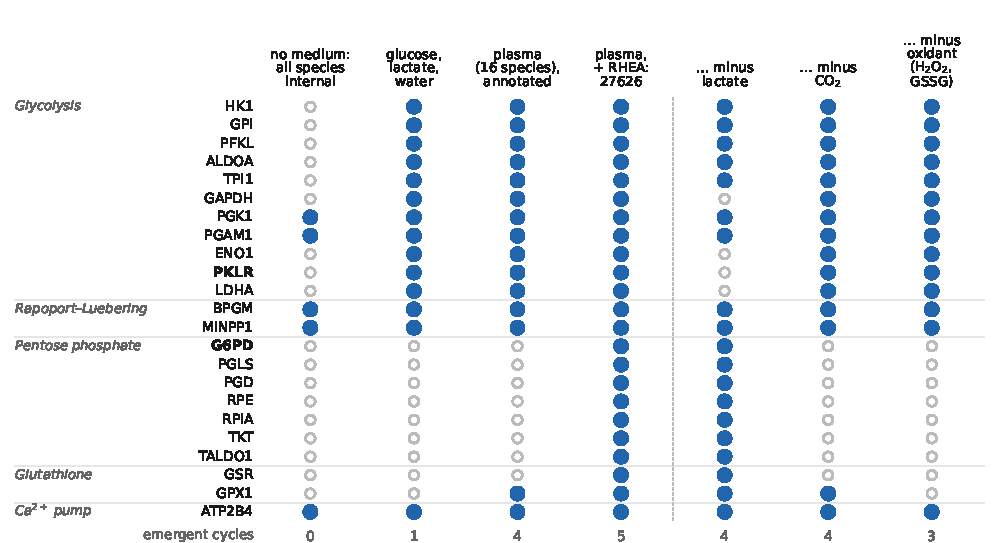
\includegraphics[width=\textwidth]{ch01_erythrocyte_cycles.pdf}
  \caption{\textbf{Which erythrocyte enzymes can carry a steady flux depends
  on what the medium holds.} Each row is an enzyme of the human red-cell
  network assembled from UniProtKB and Rhea; each column a choice of
  exchanged species. A filled circle means the enzyme lies on a cycle of
  $\ker N_{\mathcal I}$ and can carry steady flux (\Cref{c1:prop-flux}); a
  grey ring, that it lies on none and carries none. The bottom row counts
  emergent cycles. With every species internal, as in a closed flask (first
  column), pyruvate kinase (\textbf{PKLR}) and most of glycolysis lie on no
  cycle. Exchanging glucose, lactate and water puts all of glycolysis on one
  emergent cycle. With the plasma species the network contains,
  glucose-6-phosphate dehydrogenase (\textbf{G6PD}) still lies on none,
  because the annotation omits one transketolase reaction; supplied from
  Rhea (fourth column), it closes the pentose phosphate pathway. Right of the
  dashed line, one exchange is withdrawn from the fourth column at a time:
  lower glycolysis, pyruvate kinase included, needs lactate to leave,
  because the NADH made by glyceraldehyde-3-phosphate dehydrogenase can be
  reoxidised only by lactate dehydrogenase; the pentose phosphate pathway
  needs CO$_2$ to leave and an oxidant (hydrogen peroxide or glutathione
  disulfide) to enter. Ranks computed exactly over the rationals by
  \texttt{validation/ch01/medium\_closure.py}.}
  \label{c1:fig-ery}
\end{figure}

\paragraph{Which exchanges each enzyme needs.} \lnkC{} Withdrawing one
exchanged species at a time (\Cref{c1:fig-ery}, right) shows which part of
the medium each enzyme's cycles pass through. Lower glycolysis, from
glyceraldehyde-3-phosphate dehydrogenase to lactate dehydrogenase and with
pyruvate kinase in between, leaves every cycle when lactate stops leaving.
Exchanging pyruvate does not rescue it, because the NADH that
glyceraldehyde-3-phosphate dehydrogenase makes has no other route back.
Hexokinase needs glucose. Glucose-6-phosphate dehydrogenase, with the rest
of the pentose phosphate pathway and glutathione reductase, leaves every
cycle when CO$_2$ is withdrawn, and also when both oxidants, hydrogen
peroxide and glutathione disulfide, are held inside. Its only steady role in
this network is to pass oxidant from the medium, through NADPH, to
glutathione.

\paragraph{Two diseases, read with the definition.} \lnkS\lnkD{} Pyruvate
kinase deficiency is caused mostly by missense alleles that lower the
enzyme's activity~\citep{zanella2005}: a conductance change (L3) on the
cycle that every steady state of the cell needs, since it is the cell's only
net source of ATP. By \Cref{c1:thm-lesion}(a,b) the cycle and its holonomy
of $-220.6$~kJ/mol are untouched; its current falls. When ATP production
falls below the demand of the cation pumps, the cell cannot hold its
gradients, loses its shape and deformability, and is removed from the
circulation, and the patient has a chronic haemolytic
anaemia~\citep{zanella2005,grace2018}. The viability set has shrunk in every
medium; the severity is never zero.

Glucose-6-phosphate dehydrogenase deficiency is the opposite case. The
enzyme's cycles pass through the oxidant axis of the medium. In a medium
that brings in little oxidant the pathway carries little current, its loss
narrows nothing that matters, and most people with the deficiency are well
throughout life. When the medium moves along that axis---fava beans,
primaquine and some other drugs, infection---the deficient cell cannot
reduce its glutathione fast enough, and haemolysis is
acute~\citep{luzzatto2020}. That is \Cref{c1:cor-medium} in a patient: a
lesion whose severity is near zero in the usual medium and large in another,
and a disease that consists in exactly that difference. Canguilhem's
narrowed margin of tolerance has a direction here, and the network says
which.

Neither disease is visible to a test on internal cycles. Pyruvate kinase
lies on no internal cycle at all, and on the cycles where
glucose-6-phosphate dehydrogenase does lie, the holonomy is fixed by the
medium. What distinguishes the two diseases is where their reactions sit in
the cycle space through the medium, and that is what this definition reads.

%% -------------------------------------------------------------------------
\section{What the definition does not say}
\label{c1:sec-limits}
%% -------------------------------------------------------------------------

\paragraph{It needs kinetics it does not supply.} The viability set and the
margin depend on the steady-state map and the demand set of
\Cref{c1:in-steady}, which belong to a particular organism and were not
computed here. The erythrocyte check stops at the stoichiometric part of the
chain: which cycles exist and on which an enzyme lies. Lying on a cycle is
necessary for carrying flux, not sufficient, since the rank test ignores the
signs that thermodynamics imposes on each reaction.

\paragraph{Steady states are assumed unique.} Part (c) of
\Cref{c1:thm-lesion} uses uniqueness. Networks with several steady states
exist, and for them a lesion off every cycle can still move the system from
one steady state to another.

\paragraph{The medium is idealised.} \Cref{c1:in-reservoir} treats the
exchanged species as held fixed. A real medium is depleted and refilled at
finite rates, and other cells share it. For a single cell in plasma the
idealisation is good; for an organ it is not, and later chapters must widen
the system to include what this chapter calls the medium.

\paragraph{Harm is not modelled.} Wakefield's second condition, that a
dysfunction be harmful by the standards of a society~\citep{wakefield1992},
has no counterpart here. The margin is a physical quantity; whether a given
loss of it matters to a person is not, and I do not claim to derive it.

\paragraph{The postulate is assumed.} \Cref{c1:post-counted} is not derived.
If records could be made at arbitrarily small cost, the bound
$\Pi\ge\nu\theta$ would give nothing and \Cref{c1:thm-maintenance} would
lose its first step; \Cref{c1:thm-nocurrent} would not, since it uses only
the flux--force relation.

\paragraph{Data are snapshots.} The TECRDB, UniProtKB and Rhea data were
retrieved on 21 October 2026 and are archived with checksums alongside the
companion tolerance paper. Annotations change, as the transketolase gap
shows.

%% -------------------------------------------------------------------------
\section{The chain, link by link}
\label{c1:sec-ledger}
%% -------------------------------------------------------------------------

\Cref{c1:tab-ledger} collects the labels. The pattern is uneven, as it
should be: the mathematics is derived; the thermodynamics is supplied, from
results a century old; the passage to a particular cell is checked on data
where it needs only stoichiometry, and supplied from the clinical literature
where it needs more. The definitions the rest of the book refers to are
\Cref{c1:def-holonomy} (holonomy), \Cref{c1:def-emergent} (emergent cycles),
\Cref{c1:def-viability} (viability and margin), \Cref{c1:def-lesion}
(lesion) and \Cref{c1:def-disease} (disease).

\begin{table}[!t]
\centering
\small
\caption{The chain of this chapter. \lnkD{} derived here; \lnkS{} supplied,
with a reference; \lnkC{} checked on public data in
\texttt{validation/ch01/} or in the companion tolerance paper.}
\label{c1:tab-ledger}
\begin{tabular}{@{}p{4.0cm}p{8.9cm}p{2.2cm}@{}}
\toprule
Link & Content & Status\\
\midrule
Counted commitment & every record costs at least $\theta>0$ & assumed\\
Divergence, order & floored costs diverge along every selection;
  $C_M\ge M\theta$ & \lnkD\\
No self-template & a part cannot describe a whole as complex as itself
  & \lnkD\\
Individuation & separation cost at least one and monotone; identity is a
  region & \lnkD\\
Cycle space, holonomy & $Z=\ker N$; trivial holonomy if and only if exact
  & \lnkD\\
Steady flux & only reactions on a cycle of $\ker N_{\mathcal I}$ carry it
  & \lnkD\\
State function & $\Delta_rG=N^{\mathsf T}\mu$ & \lnkS\\
Internal holonomy & zero on every internal cycle, under every lesion
  & \lnkD\lnkS\\
Measured constants & internal cycle sums are measurement error (TECRDB,
  $67$ cycles) & \lnkC\\
Reservoir & the medium holds exchanged potentials fixed & \lnkS\\
Emergent holonomy & the Gibbs energy of the net exchange & \lnkD\\
Erythrocyte glycolysis & pyruvate kinase on no internal cycle; on the
  emergent cycle of $-220.6$~kJ/mol & \lnkC\\
Flux--force relation & $\ln(J^+/J^-)=-\Delta_rG/RT$ & \lnkS\\
No holonomy, no current & dissipation drawn from the medium; loop law
  & \lnkD\\
Maintenance & $\Pi\ge\nu\theta$; a living system needs emergent holonomy
  & \lnkD\lnkS\\
Viability, margin & a set of media; a margin in kJ/mol & \lnkD{}
  (kinetics \lnkS)\\
Lesions & deletion, addition, conductance change; holonomy never changes
  & \lnkD\\
Medium dependence & where a lesion acts depends on the exchanged set
  & \lnkD\lnkC\\
Annotation gap & human transketolase lacks RHEA:27626 in UniProtKB
  & \lnkC\\
Two enzymopathies & chronic against oxidant-triggered haemolysis
  & \lnkS\lnkD\\
\bottomrule
\end{tabular}
\end{table}
